% ======================================================================
% Module 3: numerical solvers and order-of-convergence check (E1)
% Three frames, no title slide: \input this file into the main deck.
%
% Needs in the main preamble:  \usepackage{graphicx,booktabs,amssymb}
% Figure is in figs/ next to this file. If this file sits in a folder
% (e.g. module3/), add \graphicspath{{module3/}} to the main preamble.
% All numbers are from report/main.tex (final Colab run).
% ======================================================================

% Shared deck colours (same values as Modules 1 and 5)
\definecolor{mvPINN}{HTML}{7B2D8E}
\definecolor{mvInk}{HTML}{1F2933}
\definecolor{mvMuted}{HTML}{5F6B7A}
\definecolor{mvSoft}{HTML}{F3EDF6}
\definecolor{mvRule}{HTML}{C9B6D3}

\providecommand{\mvTakeaway}[1]{%
  \par\vspace{3pt}\noindent
  \fcolorbox{mvRule}{mvSoft}{\parbox{\dimexpr\linewidth-2\fboxsep-2\fboxrule\relax}{\footnotesize\color{mvInk}#1}}}

% ----------------------------------------------------------------------
\begin{frame}{Two solvers written from scratch, one trusted reference}
\framesubtitle{Module 3 \textbullet\ vectorised Forward Euler and RK4 for $\dot{\mathbf y} = f(t,\mathbf y)$, $\mathbf y = (s,e,i,r,d)$}
\vspace{-2pt}
\begin{columns}[T,onlytextwidth]
\column{0.52\textwidth}
  \footnotesize\raggedright
  \textbf{\color{mvPINN}Forward Euler} {\scriptsize\color{mvMuted}one slope per step}\\[1pt]
  $\mathbf y_{k+1} = \mathbf y_k + h\, f(t_k, \mathbf y_k)$; local error $O(h^2)$, global error $O(h)$
  \vspace{5pt}

  \textbf{\color{mvPINN}Classical Runge--Kutta (RK4)} {\scriptsize\color{mvMuted}four slopes per step}
  {\scriptsize
  \[ \begin{aligned}
     k_1 &= f(t_k,\mathbf y_k), & k_2 &= f\big(t_k+\tfrac h2,\,\mathbf y_k+\tfrac h2 k_1\big),\\
     k_3 &= f\big(t_k+\tfrac h2,\,\mathbf y_k+\tfrac h2 k_2\big), & k_4 &= f(t_k+h,\,\mathbf y_k+h\,k_3)
     \end{aligned} \]}
  \vspace{-8pt}
  \[ \mathbf y_{k+1} = \mathbf y_k + \tfrac h6\,(k_1 + 2k_2 + 2k_3 + k_4) \]
  \vspace{-12pt}
  \begin{itemize}\setlength{\itemsep}{0pt}
    \item local error $O(h^5)$, global error $O(h^4)$
    \item both update all five compartments at once with NumPy arrays
  \end{itemize}
\column{0.44\textwidth}
  \footnotesize\raggedright
  \textbf{\color{mvPINN}Reference solution}
  \begin{itemize}\setlength{\itemsep}{0pt}
    \item adaptive 8th-order Dormand--Prince (\textbf{DOP853}, SciPy)
    \item rtol $3\times10^{-14}$, atol $10^{-16}$: close to the smallest SciPy accepts
  \end{itemize}
  \vspace{3pt}
  \textbf{\color{mvPINN}Why so tight?}
  \begin{itemize}\setlength{\itemsep}{0pt}
    \item a reference must be far more accurate than the solvers it judges
    \item with rtol $=10^{-12}$, RK4's error at the smallest step reaches the reference's own ($\approx10^{-12}$) and its measured order falls to \textbf{3.74}
    \item the fault is in the reference, not in RK4
  \end{itemize}
\end{columns}
\mvTakeaway{\textbf{Idea:} Euler is the simplest method (order 1), RK4 the accurate workhorse (order 4). Both orders are known in advance, so the measured slopes test the code.}
\end{frame}

% ----------------------------------------------------------------------
\begin{frame}{Two checks: conservation, and how accuracy is measured}
\framesubtitle{Module 3 \textbullet\ Experiment E1 setup: constant $\beta = 0.4858$ ($R_0 = 2$), six step sizes}
\vspace{-2pt}
\begin{columns}[T,onlytextwidth]
\column{0.47\textwidth}
  \footnotesize\raggedright
  \textbf{\color{mvPINN}Conservation of the total}
  \[ \frac{d}{dt}(s+e+i+r+d) = 0 \]
  \vspace{-12pt}
  \begin{itemize}\setlength{\itemsep}{0pt}
    \item the components of $f$ sum to zero, so every Euler or RK4 step keeps $s+e+i+r+d=1$, up to rounding
  \end{itemize}
  \vspace{2pt}
  \textbf{\color{mvPINN}Result} {\scriptsize\color{mvMuted}$t\in[0,60]$, $h \in \{1,\,0.25,\,0.03125\}$}
  \[ \max_k \Big|\sum_j y_{k,j} - 1\Big| \;\le\; 1.2\times10^{-15} \]
  \vspace{-12pt}
  \begin{itemize}\setlength{\itemsep}{0pt}
    \item a few multiples of machine epsilon ($2.2\times10^{-16}$)
    \item shows $f$ is coded consistently; it does \textbf{not} measure accuracy
  \end{itemize}
\column{0.50\textwidth}
  \footnotesize\raggedright
  \textbf{\color{mvPINN}Experiment E1}
  \begin{itemize}\setlength{\itemsep}{0pt}
    \item $\mathbf y_0 = (0.99,\,0.005,\,0.005,\,0,\,0)$ over $t\in[0,60]$ days
    \item $h = 1,\,0.5,\,0.25,\,0.125,\,0.0625,\,0.03125$ days
  \end{itemize}
  \vspace{2pt}
  \textbf{\color{mvPINN}Global error}: largest miss over all times and all five compartments
  \[ E(h) = \max_k \max_j \big| y_{k,j} - y_{\text{ref},j}(t_k) \big| \]
  \par\vspace{-2pt}
  \textbf{\color{mvPINN}Observed order}: if $E(h) \approx C h^{p}$, halving $h$ gives $p \approx \log_2\!\big[E(h)/E(h/2)\big]$; a least-squares fit of $\log E$ on $\log h$ gives one overall slope.
\end{columns}
\mvTakeaway{\textbf{Two separate questions:} conservation tests that the equations are coded consistently; convergence tests that the error shrinks at the theoretical rate.}
\end{frame}

% ----------------------------------------------------------------------
\begin{frame}{E1 result: Euler converges at order 1, RK4 at order 4}
\framesubtitle{Module 3 \textbullet\ global error against the DOP853 reference, log--log axes}
\vspace{-2pt}
\begin{columns}[T,onlytextwidth]
\column{0.49\textwidth}
  \centering
  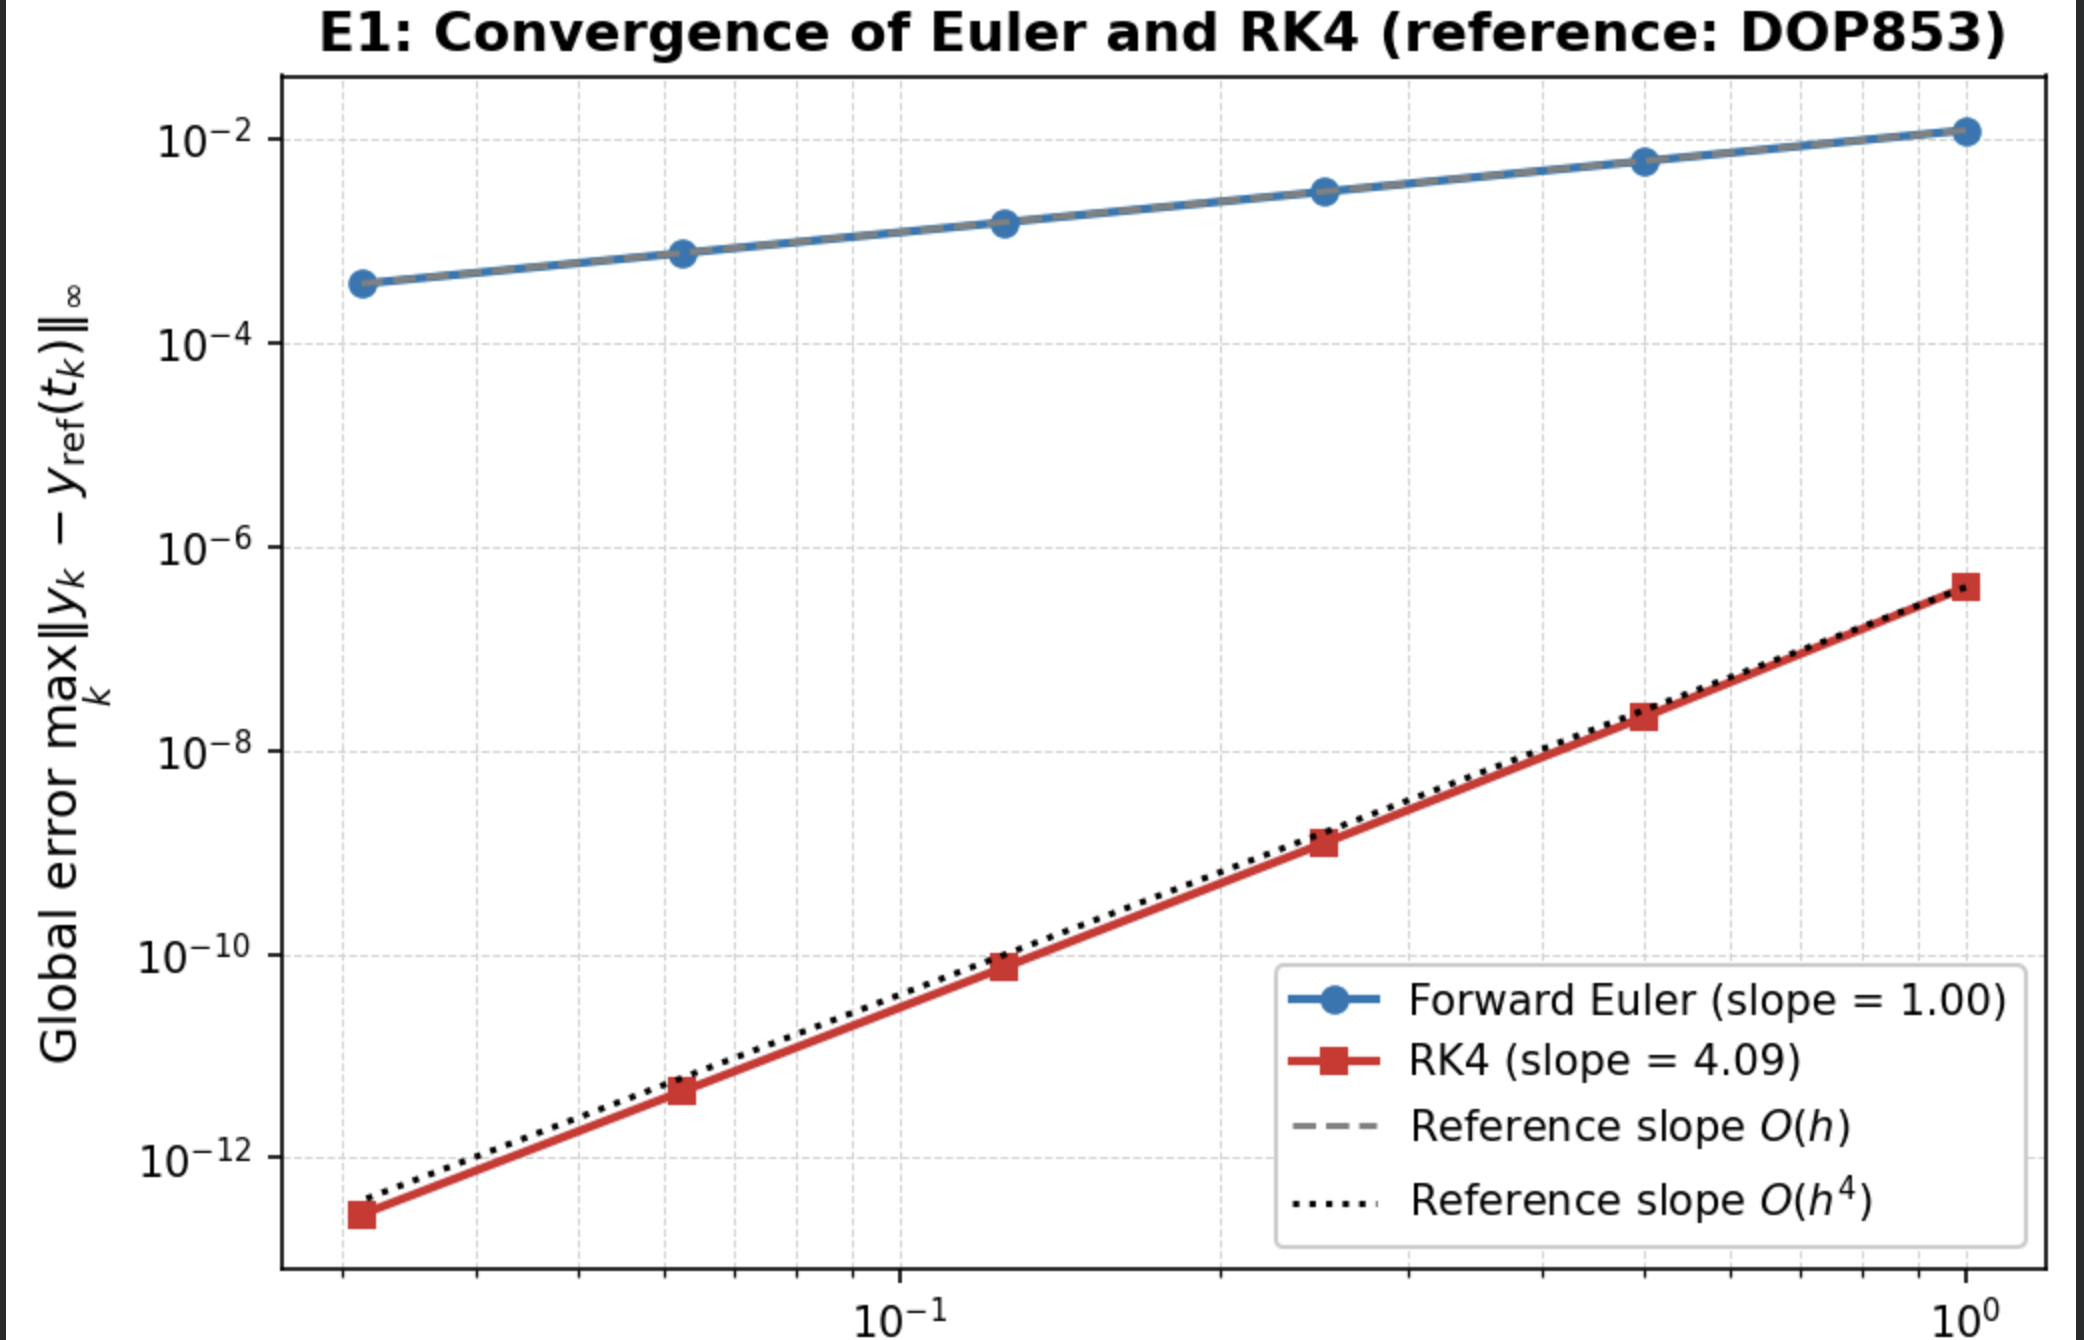
\includegraphics[height=0.50\textheight,trim=10 0 0 0,clip]{figs/fig_e1_convergence.png}\\[1pt]
  {\scriptsize\color{mvMuted} reference lines: slopes 1 and 4}
\column{0.47\textwidth}
  \scriptsize\setlength{\tabcolsep}{3.5pt}
  \begin{tabular}{@{}rcccc@{}}
    \toprule
    $h$ (days) & Euler error & order & RK4 error & order \\
    \midrule
    1       & $1.22\times10^{-2}$ & 1.004 & $4.00\times10^{-7}$  & 4.225 \\
    0.5     & $6.09\times10^{-3}$ & 1.002 & $2.14\times10^{-8}$  & 4.124 \\
    0.25    & $3.04\times10^{-3}$ & 1.001 & $1.23\times10^{-9}$  & 4.061 \\
    0.125   & $1.52\times10^{-3}$ & 1.001 & $7.34\times10^{-11}$ & 4.031 \\
    0.0625  & $7.59\times10^{-4}$ & 1.000 & $4.49\times10^{-12}$ & 4.015 \\
    0.03125 & $3.80\times10^{-4}$ & --    & $2.78\times10^{-13}$ & --    \\
    \midrule
    \multicolumn{2}{@{}l}{fitted slope} & \textbf{1.001} & & \textbf{4.085} \\
    \bottomrule
  \end{tabular}\\[3pt]
  \footnotesize\raggedright
  \begin{itemize}\setlength{\itemsep}{0pt}
    \item Euler: error \textbf{halves} when $h$ halves
    \item RK4: error falls by a factor of about \textbf{16}
    \item RK4's order sits slightly above 4 for large steps and approaches 4 as $h$ shrinks
  \end{itemize}
\end{columns}
\mvTakeaway{\textbf{Result:} observed orders 1.001 and 4.085 match the theory (1 and 4).
At $h=1$ day RK4 is about $3\times10^{4}$ times more accurate than Euler for four times the work per step, so RK4 is used for forward simulation.}
\end{frame}
